% Author: Izaak Neutelings (January 2021)
\documentclass[border=3pt,tikz]{standalone}
\usepackage{tikz}
\usetikzlibrary{arrows.meta} % to control arrow size
\tikzset{>={Latex[length=4,width=4]}} % for LaTeX arrow head
\usetikzlibrary{calc}
\usepackage{amsmath,bm}
\usepackage{relsize} % for fontsize
\usepackage{xcolor} % for colored text

\colorlet{mylightblue}{blue!5!white}
\colorlet{mydarkblue}{blue!30!black}
\colorlet{myblue}{blue!50!black}
\colorlet{myred}{red!50!black}
\colorlet{mydarkred}{red!30!black}
\colorlet{mydarkgreen}{green!30!black}


\begin{document}


% FLOW CHART
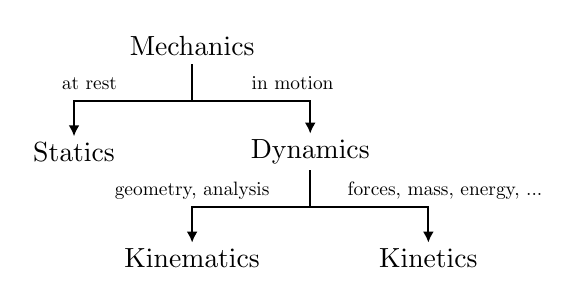
\begin{tikzpicture} %[xscale=1.3,yscale=1.3]
  \def\L{1.5}
  \def\H{2.7}
  \node[inner sep=3] %[draw=mydarkblue,thick,rounded corners=0.4,inner sep=2]
    (M) at (0,\H) {Mechanics};
  \node[inner sep=2]
    (S) at (-\L,0.5*\H) {Statics};
  \node[inner sep=2]
    (D) at (\L,0.5*\H) {Dynamics};
  \node[inner sep=2]
    (K) at (0.0*\L,0) {Kinematics};
  \node[inner sep=2]
    (k) at (2.0*\L,0) {Kinetics};
  \draw[->,thick] (M) --++ (0,-0.26*\H) -| (S)
    node[midway,left=6,above right=-1,scale=0.7] {\strut at rest}; %stationary};
  \draw[->,thick] (M) --++ (0,-0.26*\H) -| (D)
    node[midway,right=10,above left=-1,scale=0.7] {\strut in motion};
  \draw[->,thick] (D) --++ (0,-0.26*\H) -| (K)
    node[midway,left=0,above=-1,scale=0.7] {\strut geometry, analysis};
  \draw[->,thick] (D) --++ (0,-0.26*\H) -| (k)
    node[midway,right=6,above=-1,scale=0.7] {\strut forces, mass, energy, ...};
\end{tikzpicture}


\end{document}
